\documentclass[10pt]{article}

\usepackage[margin=0.68in]{geometry}
\usepackage{amsmath}
\usepackage{amssymb}
\usepackage{booktabs}
\usepackage{graphicx}
\usepackage{hyperref}
\usepackage{array}
\usepackage{enumitem}
\usepackage{caption}
\usepackage{float}

\hypersetup{colorlinks=true, linkcolor=black, citecolor=black, urlcolor=blue}
\setlist[itemize]{leftmargin=1.15em, itemsep=0.1em, topsep=0.15em}
\setlength{\parindent}{0pt}
\setlength{\parskip}{0.32em}
\captionsetup{font=small, skip=3pt}
\renewcommand{\arraystretch}{1.04}

\title{COSA+ for Robust Test-Time Adaptation in Time-Series Forecasting}
\author{Group members: Name / Student ID, Name / Student ID, Name / Student ID}
\date{}

\begin{document}
\maketitle
\vspace{-1.4em}

\begin{abstract}
Group members: Name / Student ID, Name / Student ID, Name / Student ID. This project studies test-time adaptation for long-term time-series forecasting. We reproduce the COSA output-space adapter and implement COSA+, a lightweight variant that combines richer test-time context statistics with a horizon-wise vector gate. Our research question is whether such an adapter can improve robustness when the test stream contains abrupt non-IID shifts. Experiments use DLinear on ETTh1 and Weather with clean tests, ablations, and black-swan shifts including level, variance, trend, and spike changes. The results are conditional but informative: COSA+ is not consistently better on clean short-horizon settings, yet it improves ETTh1 horizon-720 post-shift MSE against original COSA on all four synthetic shifts. On Weather, adaptation clearly beats no test-time adaptation under shifts, but the full vector gate is slightly weaker than the original adapter. These results suggest that richer adaptation can help under long-horizon abrupt shifts, while high-dimensional volatile datasets require more careful gate regularization.
\end{abstract}
\vspace{-0.8em}

\section{Introduction / Problem Definition}
Time-series forecasting models are often evaluated on fixed clean test splits. This assumption is convenient but incomplete for deployment, where streams can change because of weather events, demand shocks, financial disruptions, sensor faults, or sudden regime changes. A model that looks accurate on a clean benchmark may fail when the input and target distribution changes during inference.

This project focuses on test-time adaptation (TTA), where a trained model is adjusted using incoming test data without full retraining. We use COSA, the Context-aware Output-Space Adapter for time-series forecasting, as the baseline method. Our project is an algorithm exploration project: instead of only reproducing COSA, we ask whether extending the adapter with richer context and horizon-wise corrections improves robustness under abrupt non-IID shifts.

Our research question is: \textbf{Can COSA-style output-space adaptation remain useful when the test-time stream changes suddenly, especially at long prediction horizons?}

\section{Related Work / Background}
Recent work on time-series test-time adaptation aims to improve forecasting under non-stationarity while keeping the base model mostly frozen. COSA is the closest related method because it corrects forecasts through a lightweight context-aware output-space adapter \cite{cosa2026}. This makes it attractive for deployment because it can be attached to existing forecasting models instead of updating the full backbone. COSA still updates adapter parameters online during test-time evaluation, while our COSA+ variant studies whether richer context statistics and horizon-wise gates improve that online output-space correction.

Meta-learning and zero-shot forecasting also motivate this project. Oreshkin et al. show that forecasting models can learn transferable adaptation mechanisms across time series without retraining on each target dataset \cite{oreshkin2021meta}. Meta-TTT similarly frames test-time training through a meta-learning minimax objective \cite{tao2025metattt}. These works support the broader idea that adaptation behavior can be learned or structured before deployment rather than being treated as unrestricted online fine-tuning.

Regime-aware methods further show that forecasting performance can improve when models account for changing market or data regimes. RAM-Net uses regime-aware meta-learning to re-weight financial training samples under different market conditions \cite{jang2025ramnet}. Other time-series TTA studies show that lightweight adaptation can help under gradual distribution shifts, but aggressive online updates may hurt under noisy or unstable streams \cite{wu2026tta}. Our black-swan tests therefore inject abrupt level, variance, trend, and spike shifts into the test stream to evaluate whether recent context helps adaptation or becomes misleading near a shift boundary.

We use DLinear as the backbone because it is simple, efficient, and a strong baseline for long-term forecasting \cite{zeng2023dlinear}. The datasets follow common long-term forecasting benchmarks: ETTh1 from the ETT benchmark \cite{ett} and Weather from standard multivariate forecasting evaluations \cite{weather}.

\section{Methodology}
We compare three method families. \textbf{No-TTA} evaluates the trained DLinear model directly. \textbf{Original COSA} uses the official context-aware output-space adapter. \textbf{COSA+} is our project variant. It keeps the same backbone and evaluation pipeline, but adds richer context statistics and horizon-wise correction capacity:
\begin{itemize}
  \item \textbf{Rich context}: the adapter uses both mean-level context and volatility information from recent windows.
  \item \textbf{Vector gate}: instead of applying one coarse correction, the adapter can gate corrections by forecast step, which should matter more for long horizons.
  \item \textbf{Controlled variants}: \texttt{rich\_ctx}, \texttt{ctx\_std\_only}, and \texttt{vec\_gate} isolate which part of COSA+ changes behavior.
\end{itemize}

More concretely, original COSA applies a residual correction
\begin{equation}
  \hat{Y} = Y_{\text{base}} + \tanh(g)H,\quad
  H = W[Y_{\text{base}}; C_t] + b,
\end{equation}
where $g$ is a scalar gate and $C_t$ stores recent context means. COSA+ replaces the scalar gate with $g\in\mathbb{R}^{L}$ for step-wise correction and optionally expands $C_t$ from mean-only statistics to mean-plus-standard-deviation statistics. The adapter still starts as the identity because $g$ is initialized to zero.

For black-swan evaluation, the second part of the test stream is transformed after a shift point $T_{\text{shift}}$:
\begin{equation}
  x'_t =
  \begin{cases}
    x_t, & t < T_{\text{shift}}, \\
    S(x_t; \alpha), & t \ge T_{\text{shift}},
  \end{cases}
\end{equation}
where $S$ is one of four synthetic shifts: level, variance, trend, or spike. In the implementation, $\alpha$ is the shift magnitude, $\sigma_{\mathrm{tr}}$ is the training-set standard deviation, and $\mu_{\mathrm{pre}}=\mathrm{mean}(x_{t<T_{\text{shift}}})$.

\begin{table}[h]
\centering
\small
\caption{Synthetic black-swan shift definitions.}
\begin{tabular}{p{0.12\linewidth}p{0.52\linewidth}p{0.26\linewidth}}
\toprule
Shift type & Transformation after $T_{\text{shift}}$ & Intuition \\
\midrule
Level & $x'_t=x_t+\alpha\sigma_{\mathrm{tr}},\ t\ge T_{\text{shift}}$ & sudden mean/level change \\
Variance & $x'_t=\mu_{\mathrm{pre}}+\alpha(x_t-\mu_{\mathrm{pre}}),\ t\ge T_{\text{shift}}$ & volatility scaling around pre-shift mean \\
Trend & $x'_t=x_t+(t-T_{\text{shift}})\alpha\sigma_{\mathrm{tr}}/100,\ t\ge T_{\text{shift}}$ & gradual directional drift \\
Spike & $x'_{T_{\text{shift}}}=x_{T_{\text{shift}}}+\alpha\sigma_{\mathrm{tr}}$; otherwise unchanged & single extreme disturbance \\
\bottomrule
\end{tabular}
\label{tab:shift_definitions}
\end{table}

We report \texttt{mse\_after\_50}, the MSE after a short post-shift warm-up, to focus on recovery rather than only the exact boundary.

\section{Implementation Details}
The official implementation is kept in \path{external/COSA_ICLR2026/}. Project code is separated into \path{experiments/}, \path{experiments/tta/}, \path{experiments/blackswan/}, and \path{results/}. The main entry point is \path{experiments/run_cosa_plus.py}; black-swan shifts are implemented in \path{experiments/blackswan/shift_injector.py} and \path{experiments/blackswan/run_blackswan.py}. Final tables and figures are stored in \path{results/final_figures/}.

The tested environment uses Python 3.10.20, PyTorch 2.11.0+cu128, NumPy 1.23.5, SciPy 1.10.1, and an NVIDIA GeForce RTX 5090 GPU. We also added preflight checks so experiments fail clearly when required datasets or checkpoints are missing, instead of silently evaluating randomly initialized models.

\section{Experiments}
We evaluate DLinear on ETTh1 and Weather. Clean-test experiments use horizons 96, 192, 336, and 720 when checkpoints are available. Ablations compare original COSA with COSA+ components. Black-swan experiments use horizon 720 and shift magnitude 3.0 for level, variance, trend, and spike shifts.

Metrics are MSE and MAE for clean tests, plus \texttt{mse\_after\_50} for shifted tests. Lower values are better. For comparisons against a baseline, relative improvement is computed as
\begin{equation}
\frac{\text{Baseline MSE} - \text{Method MSE}}{\text{Baseline MSE}} \times 100\%.
\end{equation}

\section{Results and Analysis}
\begin{table}[H]
\centering
\small
\caption{Clean-test MSE for original COSA and COSA+. Lower is better.}
\begin{tabular}{lrrr}
\toprule
Dataset & Horizon & Original COSA & COSA+ \\
\midrule
ETTh1 & 96 & \textbf{0.452734} & 0.453148 \\
ETTh1 & 192 & \textbf{0.501868} & 0.502388 \\
ETTh1 & 336 & 0.547112 & \textbf{0.546639} \\
ETTh1 & 720 & 0.673144 & \textbf{0.670793} \\
Weather & 96 & \textbf{0.190825} & 0.191509 \\
Weather & 720 & \textbf{0.344698} & 0.349111 \\
\bottomrule
\end{tabular}
\label{tab:clean}
\end{table}

Table~\ref{tab:clean} shows that COSA+ is not a universal clean-test improvement. It is slightly worse than original COSA at ETTh1 horizons 96 and 192, but becomes better at horizons 336 and 720. This supports our hypothesis only conditionally: horizon-wise correction is more useful when forecast errors propagate across many future steps. On Weather, COSA+ is worse in MSE, suggesting that the full vector-gate design is sensitive to high-variance multivariate data.

\begin{table}[H]
\centering
\small
\caption{ETTh1 DLinear ablation MSE. Lower is better.}
\begin{tabular}{rrrrrr}
\toprule
Horizon & Original & VecGate & RichCtx & StdOnly & COSA+ \\
\midrule
96 & \textbf{0.452734} & 0.452959 & 0.452891 & 0.452863 & 0.453148 \\
192 & \textbf{0.501868} & 0.502159 & 0.502122 & 0.502110 & 0.502388 \\
336 & 0.547112 & \textbf{0.546485} & 0.547067 & 0.547069 & 0.546639 \\
720 & 0.673144 & 0.670848 & 0.672205 & 0.672253 & \textbf{0.670793} \\
\bottomrule
\end{tabular}
\label{tab:ablation}
\end{table}

The ablation in Table~\ref{tab:ablation} explains the clean ETTh1 pattern. The vector gate is not useful at short horizons, but it becomes the main source of improvement at horizons 336 and 720. Rich context alone is stable but small. Therefore, the main benefit of COSA+ comes from forecast-step-specific correction capacity, not just adding more statistics.

\begin{figure}[H]
\centering
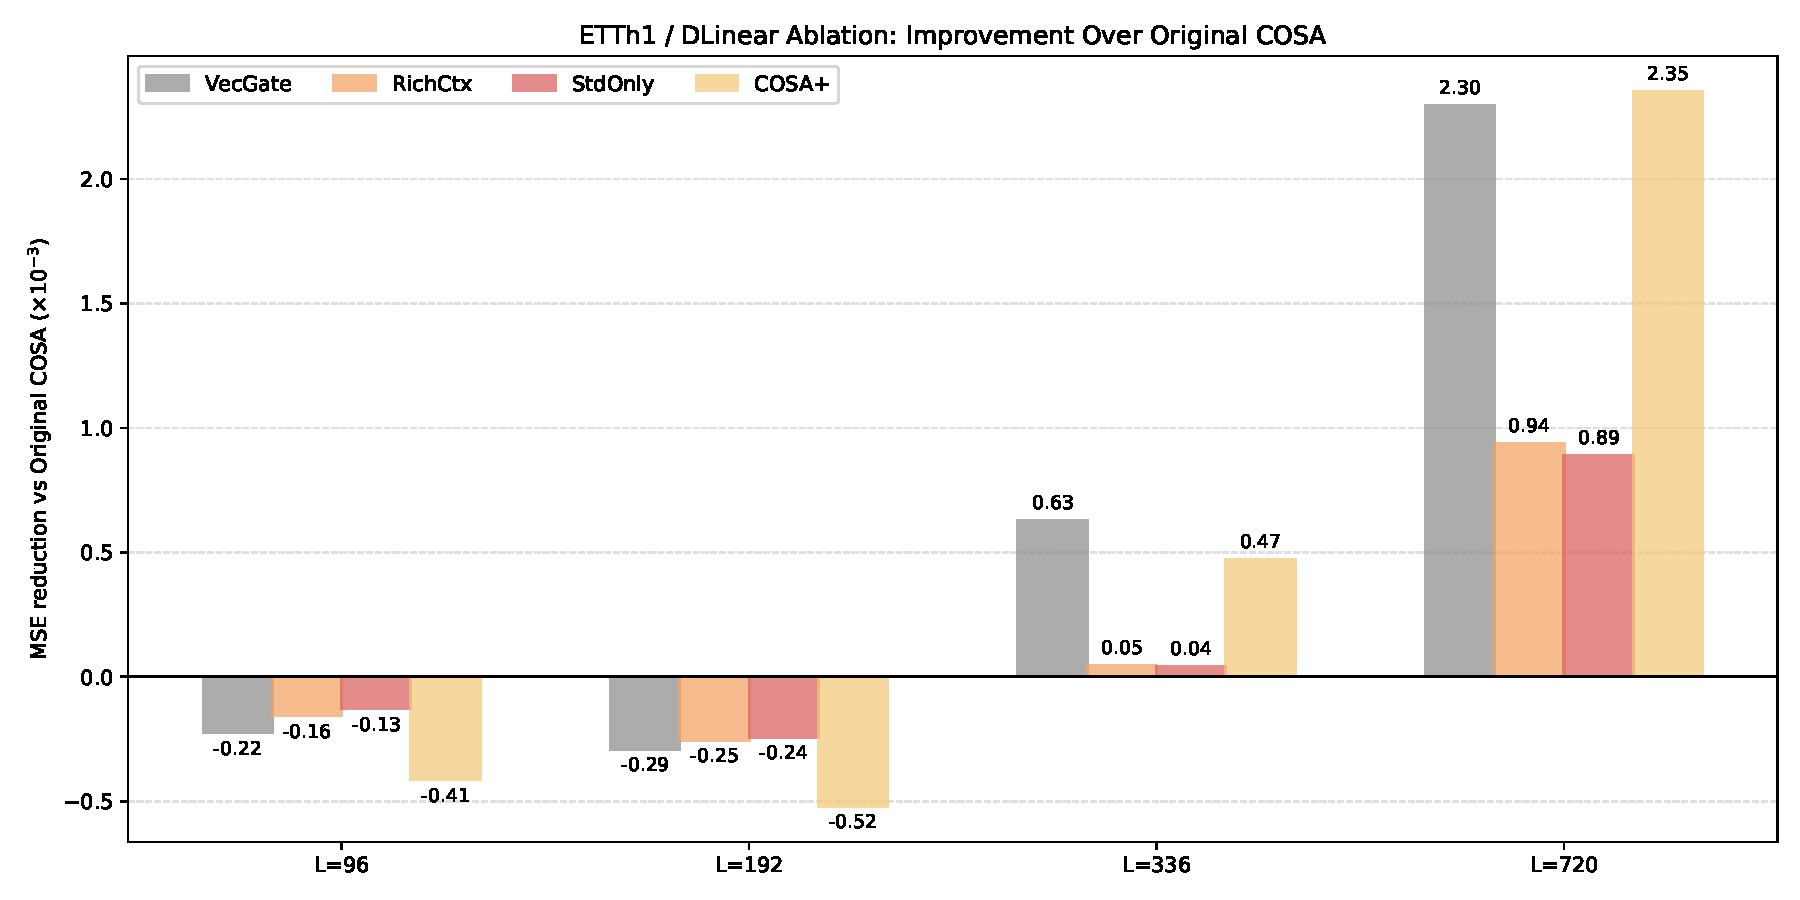
\includegraphics[width=0.82\linewidth]{../../results/final_figures/figure2_etth1_ablation_bar.pdf}
\caption{ETTh1 ablation trend. COSA+ is most useful at the longest horizon.}
\label{fig:ablation}
\end{figure}

\begin{figure}[H]
\centering
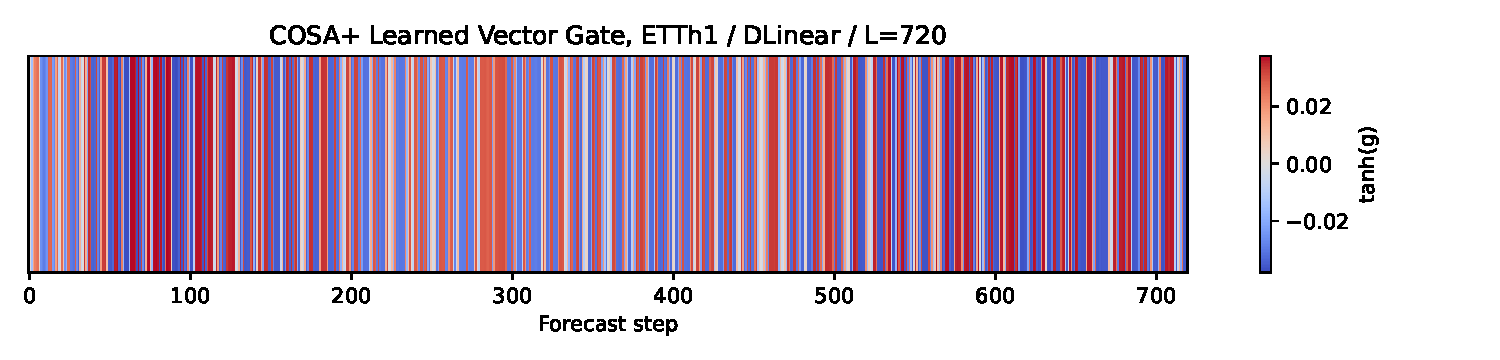
\includegraphics[width=0.72\linewidth]{../../results/final_figures/figure3_gate_heatmap_etth1_h720.pdf}
\caption{Learned COSA+ vector gate on ETTh1 horizon 720. Non-uniform values indicate that the adapter learns different correction strengths across forecast steps.}
\label{fig:gate}
\end{figure}

\begin{table}[H]
\centering
\small
\caption{Black-swan ETTh1 horizon-720 \texttt{mse\_after\_50}. Lower is better.}
\begin{tabular}{lrrr}
\toprule
Shift & No-TTA & Original COSA & COSA+ \\
\midrule
Level & 1.5141 & 1.3900 & \textbf{1.3707} \\
Variance & 1.4018 & 1.3126 & \textbf{1.3033} \\
Trend & 1.0925 & 0.9965 & \textbf{0.9854} \\
Spike & 1.0715 & 0.9798 & \textbf{0.9699} \\
\bottomrule
\end{tabular}
\label{tab:etth1_shift}
\end{table}

Table~\ref{tab:etth1_shift} gives the strongest positive result. At horizon 720, both COSA methods beat no-TTA after abrupt shifts, and COSA+ is best for all four shift types. Relative to original COSA, COSA+ improves post-shift MSE by about 0.95\%--1.39\%. Relative to no-TTA, the gain is much larger, around 9\%--10\%. This indicates that output-space adaptation is useful after the shift, and the added horizon-wise flexibility helps long-horizon recovery.

\begin{table}[H]
\centering
\small
\caption{ETTh1 horizon-720 black-swan ablation at shift magnitude 3.0. Values are \texttt{mse\_after\_50}; lower is better.}
\begin{tabular}{lrrrr}
\toprule
Shift & Original COSA & VecGate & RichCtx & COSA+ \\
\midrule
Level & 1.3900 & 1.3716 & 1.3894 & \textbf{1.3707} \\
Variance & 1.3126 & 1.3037 & 1.3125 & \textbf{1.3033} \\
Trend & 0.9965 & 0.9858 & 0.9964 & \textbf{0.9854} \\
Spike & 0.9798 & 0.9703 & 0.9797 & \textbf{0.9699} \\
\bottomrule
\end{tabular}
\label{tab:etth1_shift_ablation}
\end{table}

\begin{figure}[H]
\centering
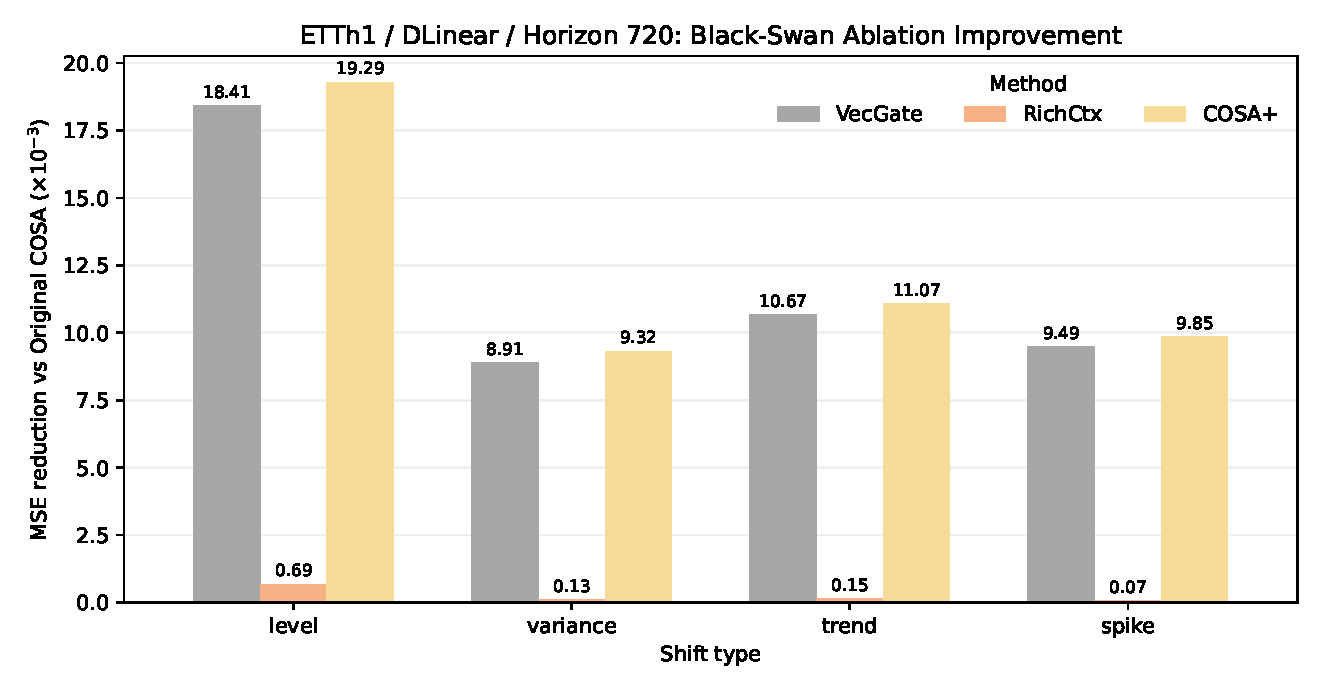
\includegraphics[width=0.82\linewidth]{../../results/final_figures/figure_etth1_blackswan_ablation_h720_mag3_bar_v2.pdf}
\caption{ETTh1 horizon-720 black-swan ablation improvement at shift magnitude 3.0. Values show MSE reduction relative to Original COSA; higher is better. COSA+ is nearly tied with VecGate and clearly better than RichCtx.}
\label{fig:etth1_shift_ablation}
\end{figure}

Table~\ref{tab:etth1_shift_ablation} and Figure~\ref{fig:etth1_shift_ablation} explain where the black-swan gain comes from. COSA+ is very close to the VecGate-only variant across all four shift types, while RichCtx remains close to original COSA. This suggests that the post-shift improvement mainly comes from the horizon-wise vector gate, which can adjust correction strength across forecast steps, rather than from richer context statistics alone.

\begin{figure}[H]
\centering
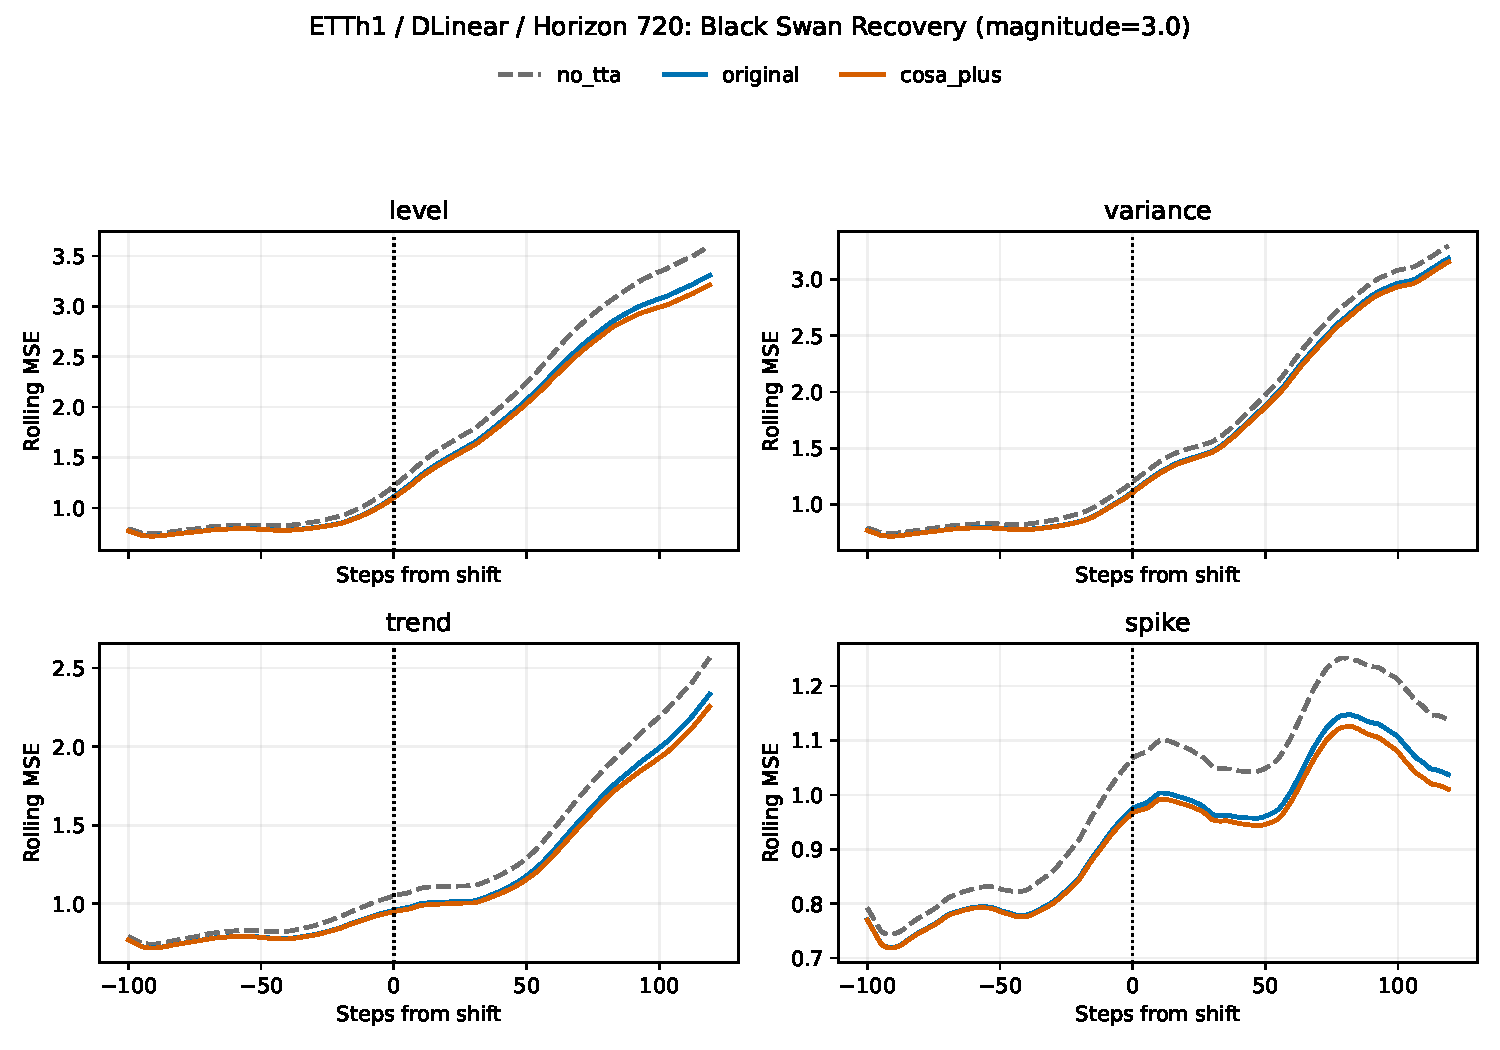
\includegraphics[width=0.82\linewidth]{../../results/final_figures/figure1_etth1_h720_blackswan_recovery.pdf}
\caption{ETTh1 horizon-720 black-swan recovery across shift types.}
\label{fig:recovery}
\end{figure}

\begin{table}[H]
\centering
\small
\caption{Weather horizon-720 black-swan \texttt{mse\_after\_50}. Lower is better.}
\begin{tabular}{lrrrr}
\toprule
Shift & No-TTA & Original & RichCtx & COSA+ \\
\midrule
Level & 0.5340 & \textbf{0.4633} & 0.4634 & 0.4665 \\
Variance & 0.2244 & 0.2065 & \textbf{0.2062} & 0.2066 \\
Trend & 0.2065 & \textbf{0.1614} & 0.1614 & 0.1626 \\
Spike & 0.2021 & 0.1606 & \textbf{0.1606} & 0.1617 \\
\bottomrule
\end{tabular}
\label{tab:weather_shift}
\end{table}

Weather gives a more cautious conclusion. Adaptation is clearly valuable under shifts: original COSA reduces post-shift MSE by about 8\% on variance shift and more than 20\% on trend/spike shifts compared with no-TTA. However, the full COSA+ variant is slightly worse than original COSA. The rich-context-only variant is almost tied with original and slightly best on variance/spike. A plausible reason is dataset dimensionality: ETTh1 has 7 variables, while Weather has 21 variables. COSA adapts variable-wise output streams, so the adaptation signal is spread across more parallel univariate streams on Weather. With only $S=3$ gradient steps per batch, the 720-dimensional vector gate may not receive enough stable signal to learn useful step-wise corrections. This separates the two modifications: Mod B (rich context) is stable, while Mod A (vector gating) needs stronger regularization or dataset-specific tuning on high-dimensional volatile data.

As supporting sensitivity evidence, we also swept black-swan magnitude on ETTh1/DLinear at horizon 720 for magnitudes 1.0, 2.0, and 3.0. COSA+ beats original COSA in all 12 shift-magnitude settings, while both adaptation methods remain better than no-TTA. The sweep supports the robustness trend, especially for level and variance shifts where error increases most strongly with magnitude, but we treat it as supporting evidence because it covers one dataset, backbone, and horizon.

\begin{figure}[H]
\centering
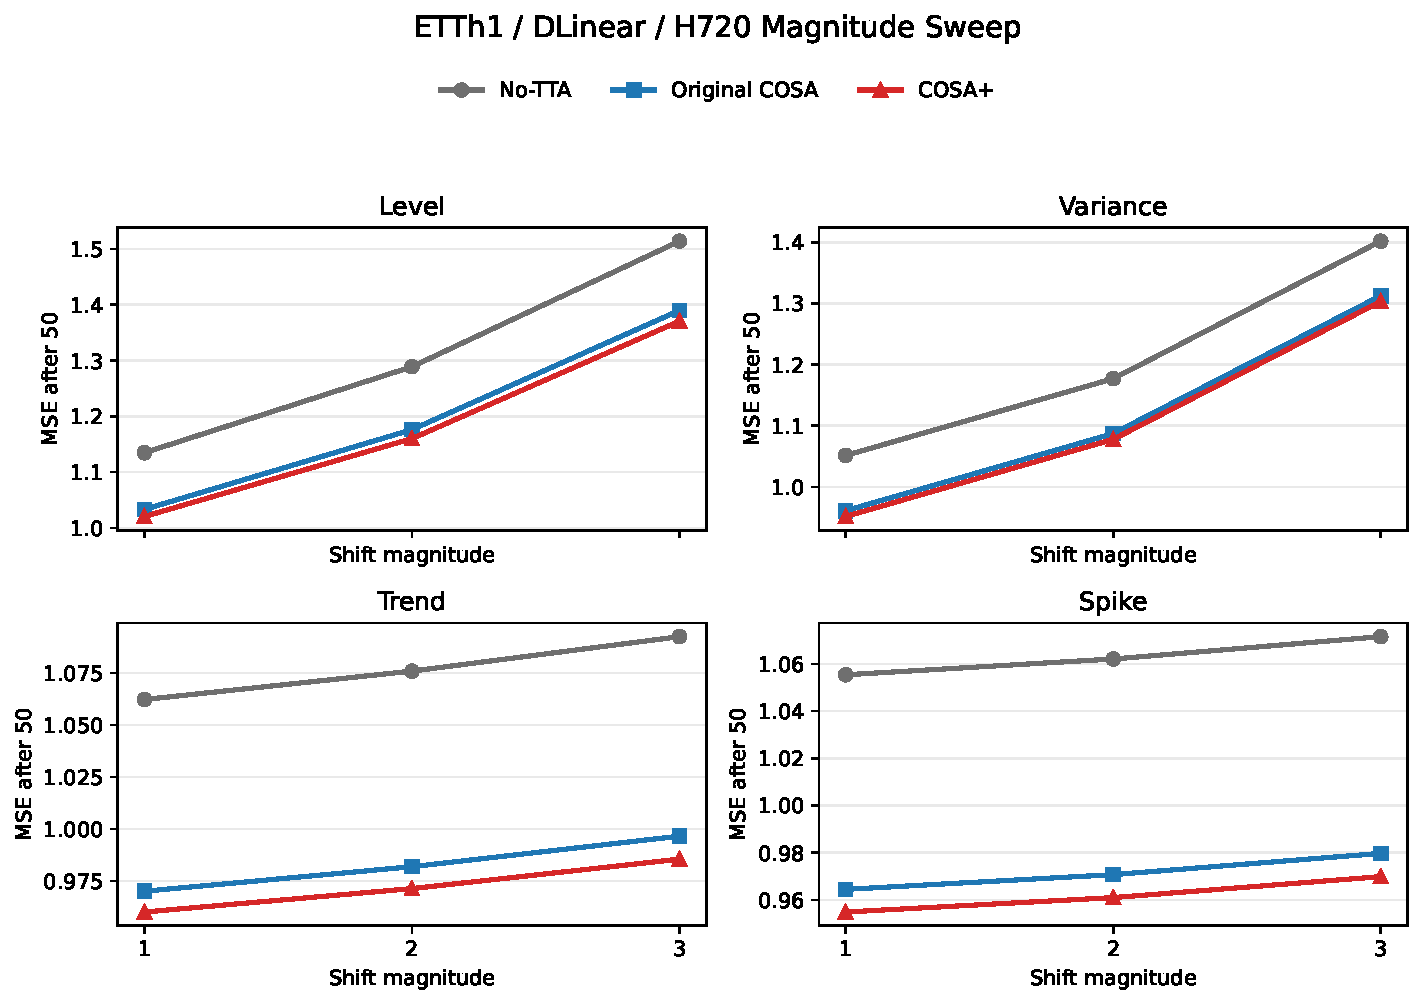
\includegraphics[width=0.88\linewidth]{../../results/final_figures/figure_etth1_blackswan_magnitude_sweep_h720_clear_v1.pdf}
\caption{Supporting magnitude sweep on ETTh1/DLinear horizon 720. COSA+ consistently improves over original COSA across all 12 shift-magnitude settings.}
\label{fig:magnitude_sweep}
\end{figure}

\section{Conclusion}
This project reproduced COSA and explored COSA+ for robust test-time adaptation in time-series forecasting. The main finding is conditional rather than absolute. COSA+ does not reliably improve clean short-horizon performance, and on Weather the full vector gate can hurt. However, at ETTh1 horizon 720 under abrupt black-swan shifts, COSA+ consistently improves over original COSA and no-TTA, and the black-swan ablation shows that this gain mainly comes from the horizon-wise vector gate rather than richer context statistics alone. The result supports the idea that richer output-space adaptation is most useful when the forecast horizon is long and post-shift errors accumulate over many future steps. The limitation is equally important: high-dimensional Weather results show that vector gating should not be treated as a free improvement. Future work should tune gate regularization, add explicit shift detection, and test whether adaptive gate freezing helps volatile multivariate datasets.

\clearpage
\begin{thebibliography}{9}
\bibitem{cosa2026}
J. Im and H.-Y. Kwon. COSA: Context-aware output-space adapter for test-time adaptation in time series forecasting. \textit{International Conference on Learning Representations (ICLR)}, 2026.

\bibitem{oreshkin2021meta}
Boris N. Oreshkin, Dmitri Carpov, Nicolas Chapados, and Yoshua Bengio. Meta-learning framework with applications to zero-shot time-series forecasting. \textit{Proceedings of the AAAI Conference on Artificial Intelligence}, 2021. \url{https://arxiv.org/pdf/2002.02887}

\bibitem{jang2025ramnet}
J. Jang, T. Kim, D. Oh, and S.-H. Park. Adaptive sample weighting with regime-aware meta-learning framework for financial forecasting. In \textit{Proceedings of the 6th ACM International Conference on AI in Finance (ICAIF '25)}, ACM, 2025. \url{https://doi.org/10.1145/3768292.3770374}

\bibitem{tao2025metattt}
Chen Tao, Li Shen, and Soumik Mondal. Meta-TTT: A meta-learning minimax framework for test-time training. \textit{International Conference on Machine Learning and Applications (ICMLA)}, 2025. \url{https://doi.org/10.1109/ICMLA66185.2025.00008}

\bibitem{wu2026tta}
Yurui Wu, Qingying Deng, Wonou Chung, and Mairui Li. Test-time adaptation for non-stationary time series: From synthetic regime shifts to financial markets, 2026. \url{https://arxiv.org/pdf/2602.00073}

\bibitem{cosa_repo}
BigBases. COSA\_ICLR2026: Official implementation of COSA. GitHub repository. \url{https://github.com/bigbases/COSA_ICLR2026}

\bibitem{zeng2023dlinear}
Ailing Zeng, Muxi Chen, Lei Zhang, and Qiang Xu. Are Transformers Effective for Time Series Forecasting? \textit{Proceedings of the AAAI Conference on Artificial Intelligence}, 2023. \url{https://arxiv.org/abs/2205.13504}

\bibitem{ett}
Zhou Tian. ETDataset: Electricity Transformer Temperature benchmark datasets. GitHub repository. \url{https://github.com/zhouhaoyi/ETDataset}

\bibitem{weather}
Haixu Wu, Jiehui Xu, Jianmin Wang, and Mingsheng Long. Autoformer: Decomposition Transformers with Auto-Correlation for Long-Term Series Forecasting. \textit{NeurIPS}, 2021. \url{https://arxiv.org/abs/2106.13008}
\end{thebibliography}

\section*{AI Usage Statement}
We used AI tools to help understand the course requirements, inspect and organize the codebase, debug experiment scripts, generate LaTeX report drafts, and improve writing clarity. All experimental design choices, implementation changes, numerical results, result analysis, and final conclusions should be reviewed and verified by the project members before submission.

\section*{Team Contribution Statement}
Fill in the actual names, student IDs, and contributions before submission.
\begin{itemize}
  \item Member A, student ID: environment setup, COSA reproduction, result collection.
  \item Member B, student ID: COSA+ implementation, ablation design, black-swan shift experiments.
  \item Member C, student ID: result analysis, report writing, presentation preparation.
\end{itemize}

\section*{Appendix: Reproducibility Notes}
Main scripts used in this project include:
\begin{itemize}
  \item \path{experiments/run_05_main_exp.sh}
  \item \path{experiments/run_04_ablation.sh}
  \item \path{experiments/run_06_blackswan_mag3.sh}
  \item \path{experiments/run_07_blackswan_etth1_ablation.sh}
  \item \path{experiments/run_08_blackswan_magnitude_sweep.sh}
  \item \path{experiments/make_final_artifacts.py}
  \item \path{experiments/blackswan/make_small_artifacts.py}
\end{itemize}
The final report figures and tables are stored under \path{results/final_figures/}.

\end{document}
